%%%%%%%%%%%%%%%%%%%%%%%%%%%%%%%%%%%%%%%%%%%%%%%%%%%%%%%%%%%%%%%%%%%%%%%%
%                                                                      %
%     File: Thesis_Appendix_A.tex                                      %
%     Tex Master: Thesis.tex                                           %
%                                                                      %
%     Author: Andre C. Marta                                           %
%     Last modified :  2 Jul 2015                                      %
%                                                                      %
%%%%%%%%%%%%%%%%%%%%%%%%%%%%%%%%%%%%%%%%%%%%%%%%%%%%%%%%%%%%%%%%%%%%%%%%

\chapter{How to control and set the desired V-F pair - rocm-smi}
\label{chapter:appendixRocm-smi}

As introduced in this dissertation, the independent control of frequency and voltage is not widely available, and only recently, AMD allows it through their ROCm software stack, more specifically through rocm-smi - ROCm system management interface. However, even the most recent version of this tool (presented on ROCm 3.8) does not provide an easy and utterly understandable way of setting the desired frequency and voltage pair. This Annex intends to describe how to command the rocm-smi tool to control and set the desired V-F pair in the two tested GPUs, AMD Vega 10 Frontier Edition and AMD Radeon 5700 XT.

As described in Chapter 2, rocm-smi is a Linux command line application. When launch, it prompts the interface exhibited in Figure~\ref{fig:rocm-smi} where it is possible to check the device temperature, average device power, core domain clock - \texttt{sclk}, \acrshort{dvfs} domain clock - \texttt{mclk}, percentage of fan speed, \texttt{perf} - indicating current DVFS setting as automatic or manual, current device power cap and finally, DRAM and Core utilization.

\begin{figure}[htb]
    \centering
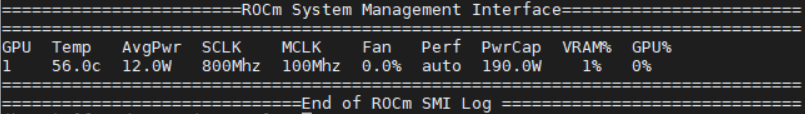
\includegraphics[width=0.75\textwidth]{Figures/AnnexA/rocm-smi.png}
        \caption{Rocm-smi interface.}
    \label{fig:rocm-smi}
\end{figure}


The V-F settings' control depends on the current device underuse due to different implementations of their \acrshort{dvfs} system. However, \texttt{perf} configuration and device power cap have to be changed regardless of the implementation of the \acrshort{dvfs} system. 

The following enumeration describes the steps to be made regardless of the implementation of the \acrshort{dvfs} system, stressing the reasons for the same. The following sections detail the working and tunning of the V-F pair for each of the tested \acrshort{gpu}s.

\begin{enumerate}
\item \textbf{Change device performance level:} Disable automatic \acrshort{dvfs} system.\\
\texttt{rocm-smi --setperflevel manual}
\item \textbf{Get device maximum power cap:} Get maximum allowed power consumption (PowerCap) allowed by the device. \\
\texttt{rocm-smi --showmaxpower} 
\item \textbf{Change device power cap:} Change the current device maximum power consumption to the value obtained on the previvous command.\\
\texttt{rocm-smi --setpoweroverdrive X --autorespond yes}
\end{enumerate}

It is necessary to change the default PowerCap value to fully unlock manual tunning of the \acrshort{dvfs} system. If not changed, the device will not allow sustained configuration of the highest frequency and voltage levels.

\section{AMD Vega 10 Frontier Edition}

The Vega 10 \acrshort{gpu} presents the concept of discrete performance levels, containing eight possible configurations for the core \acrshort{dvfs} domain. 
When editing the frequency and voltage values of each performance level, three rules must be followed. If that is not the case, even though the system accepts the configuration, the \texttt{perf} configuration (performance level) switches to automatic. The rules are 

\begin{enumerate}
\item the desired frequency and voltage values must be within the valid ranges for the target device; 
\item the desired frequency and voltage values cannot have the same value as the default for the given performance level; 
\item the selected frequency and voltage values of the performance level $i$ need to be at least 1 unit (1 MHz or 1 mV) above the performance level $i-1$ and one unit below the performance level $i+1$.
\end{enumerate}

To guarantee that the desired V-F pair is selected, it is necessary to write on performance level 0 to 6 V-F pairs below all configurations that will be used and apply on the performance level 7 the desired V-F pair. In this way, even some automatic control systems that may remain active are forced to select the wanted configuration. Table~\ref{tab:gpulevels-tunning} presents the pre-defined voltage values for the performance levels.

\begin{table}[!htb]
\centering
\begin{tabular}{ccc}
\textbf{Level} & \textbf{Frequency {[}MHz{]}} & \textbf{Voltage {[}mV{]}}  \\ \hline
0              & 853                          & 801                        \\
1              & 860                          & 810                      \\
2              & 870                          & 820                       \\
3              & 880                          & 830                      \\ 
4              & 890                          & 840                      \\
5              & 900                          & 850                     \\
6              & 910                          & 860                       \\
7              & \texttt{Desired Frequency}   & \texttt{Desired Voltage}                     \\ \hline
\end{tabular}
\caption{Vega 10 GPU core performance levels general configuration.}
\label{tab:gpulevels-tunning}
\end{table}

The following enumeration indicates the rocm-smi commands that should be executed to select the desired voltage-frequency configuration.

\begin{enumerate}
\setcounter{enumi}{3}
\item \textbf{Change performance levels 0 to 6 to pre defined values:} \\
\texttt{rocm-smi --setslevel 0 853 801 --autorespond yes}\\
\texttt{rocm-smi --setslevel 1 860 810 --autorespond yes}\\
\texttt{rocm-smi --setslevel 2 870 820 --autorespond yes}\\
\texttt{rocm-smi --setslevel 3 880 830 --autorespond yes}\\
\texttt{rocm-smi --setslevel 4 890 840 --autorespond yes}\\
\texttt{rocm-smi --setslevel 5 900 850 --autorespond yes}\\
\texttt{rocm-smi --setslevel 6 910 860 --autorespond yes}
\item \textbf{Change performance levels 7 to desired values:} \\
\texttt{rocm-smi --setslevel 7 \$frequency \$voltage --autorespond yes}
\item \textbf{Select core performance level 7:} \\
\texttt{rocm-smi --setsclk 7 --autorespond yes}
\item \textbf{Confirm the current voltage level:} To note that this command shows the voltage value that corresponds to $max(V_{Core}, V_{DRAM})$, so, if a voltage value is selected on the core domain is smaller than the current applied on the \acrshort{dram} domain, the tool will report the voltage value of the \acrshort{dram} domain.\\
\texttt{rocm-smi --showvoltage}
\end{enumerate}




\section{AMD Radeon 5700 XT}

The Radeon 5700 XT \acrshort{dvfs} system does not present the concept of performance levels. Instead, three V-F pairs indicated, and a quadratic regression is made to create the function $V(f)$ (chart presented in Chapter 2 Figure~\ref{fig:voltage_curve}). Similarly to the Vega 10 \acrshort{gpu}, the three V-F pairs also need to respect the three indicated rules.

\begin{figure}[htb]
    \centering
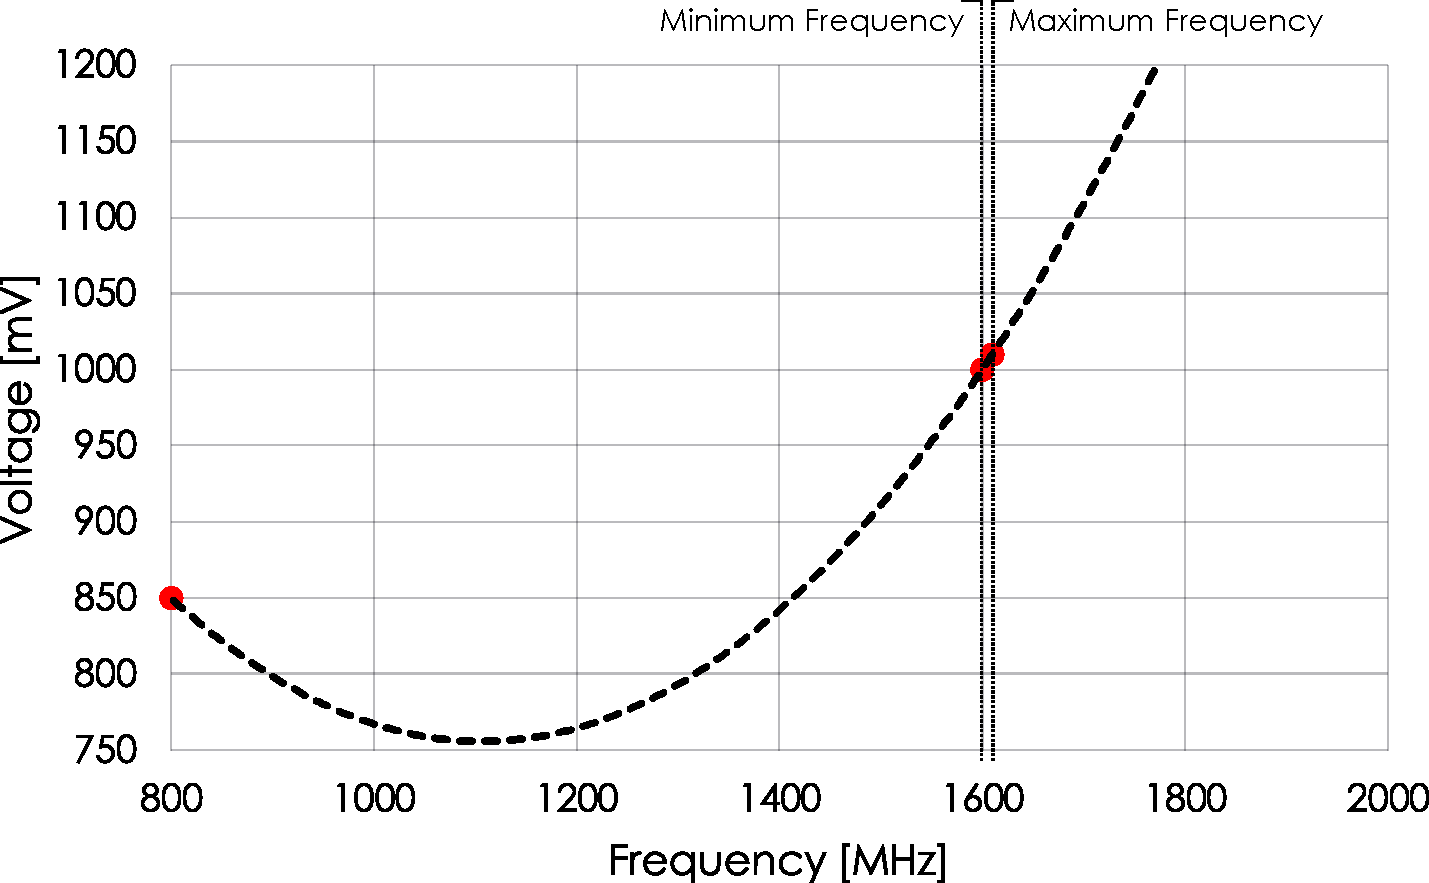
\includegraphics[width=0.75\textwidth]{Figures/AnnexA/vegadvfscontrol.pdf}
        \caption{Change in voltage curve to select a given V-F pair.}
    \label{fig:voltagecurvepair}
\end{figure}

Overall, to be able to select and apply a specific V-F pair, the rocm-smi interface presents one other command that indicates to the \acrshort{dvfs} system, which is the minimum and maximum frequency that should be used. Taking advantage of that interface, the devised method to select a given frequency is presented in Figure~\ref{fig:voltagecurvepair}, where the first V-F pair is not changed, and the remaining two are set following Table~\ref{tab:xt-pairs}. The value of $+10$ is the pre-defined allowed variation of the parameters and was decided taking into account the range of frequency and voltage values.



\begin{table}[!htb]
\centering
\begin{tabular}{ccc}
\textbf{V-F pair number} & \textbf{Frequency {[}MHz{]}} & \textbf{Voltage {[}mV{]}}  \\ \hline
0              & 800                          & 850                        \\
1              & \texttt{Desired Frequency}   & \texttt{Desired Voltage}                        \\
2              & \texttt{Desired Frequency} + 10   & \texttt{Desired Voltage} + 10                        \\\hline
\end{tabular}
\caption{Radeon 5700 XT GPU core V-F pairs general configuration.}
\label{tab:xt-pairs}
\end{table}


The following enumeration indicates the rocm-smi commands that should be executed to select the desired voltage-frequency configuration.

\begin{enumerate}
\setcounter{enumi}{3}
\item \textbf{Change the V-F pair values:} \\
\texttt{rocm-smi --setvc 0 800 850  --autorespond yes}\\
\texttt{rocm-smi --setvc 1 \$frequency \$voltage     --autorespond yes}\\
\texttt{rocm-smi --setvc 2 \$\{frequency + 10\} \$\{voltage + 10\}  --autorespond yes}
\item \textbf{Change allowed frequency range limits:} \\
\texttt{rocm-smi --setsrange 0 \$frequency --autorespond yes}\\
\texttt{rocm-smi --setsrange 1 \$\{frequency + 10\} --autorespond yes}
\item \textbf{Confirm the current voltage level:} To note that this command shows the voltage value that corresponds to $max(V_{Core}, V_{DRAM})$, so, if a voltage value is selected on the core domain is smaller than the current applied on the \acrshort{dram} domain, the tool will report the voltage value of the \acrshort{dram} domain.\\
\texttt{rocm-smi --showvoltage}
\end{enumerate}

